\documentclass{minimal}

\usepackage{graphicx}
\usepackage{stackengine}
\usepackage{tikz}
\usetikzlibrary{positioning}
\usetikzlibrary{shapes.geometric}
\usetikzlibrary{calc}
%% \usetikzlibrary{arrows}
\usetikzlibrary{arrows.meta}
%% \tikzset{%
%%   strongT/.tip={Triangle},/.style={line width=12mm}
%% }
\newcommand\vcdots{\;\stackMath\stackinset{c}{0pt}{c}{0.6ex}{\vdots}{\vphantom{-}}\;}
%% \setstackgap{S}{inter-item stackgap}
%% \setstackgap{L}{1.2em}

\begin{document}

\tikzset{every picture/.style={line width=0.9pt}}

%% \begin{figure}[p] % remove when finished
\hspace*{-80pt}\begin{tikzpicture}[
networknode/.style={regular polygon,regular polygon sides=4, draw=black, fill=none, ultra thick, inner sep=-7pt},
vectornode/.style={rectangle, draw=black, fill=none, },
internode/.style={rectangle, draw=black, fill=none, thick},
imagenode/.style={rectangle, draw=none, fill=none},
>={Triangle[width=2.2mm,length=2.0mm]},->
]

%Nodes
% What sorta style should the text have? Blue ass well?
% mention a cnn somewhere
% also see https://www.researchgate.net/figure/The-high-level-concept-of-an-extended-variational-autoencoder-adopted-for_fig8_317486066
% http://bjlkeng.github.io/images/variational_autoencoder2.png
\node[imagenode] (input) [] [label=below:{$X$}]{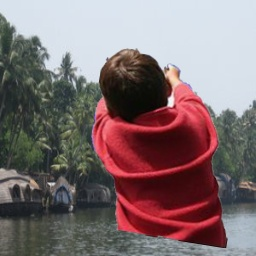
\includegraphics[width=0.1\textwidth]{syn1}};
\node[networknode] (encoder) [right=of input][label=below:{\mbox{$Q(z|X)$}}]
     [label=above:{\textit{Convolutions}}]{\textbf{Encoder Network}};
\node[right=1.5cm of encoder] (dummy) {}; 
\node[internode] (mean) [below=of dummy] {$\mu(X)$};
\node[internode] (std) [above=of dummy] {$\Sigma(X)$};
\node[vectornode] (latent) [right=1.5cm of dummy] {\Vectorstack{{z_1} {\vcdots} {z_n}}};
\node[networknode] (decoder) [right=1.08cm of latent][label=below:{\mbox{$P(X|z)$}}]
     [label=above:{\textit{Transposed Convolutions}}]{\textbf{Decoder Network}};
\node[imagenode] (output) [right=of decoder][label=below:$\widetilde{X}$] {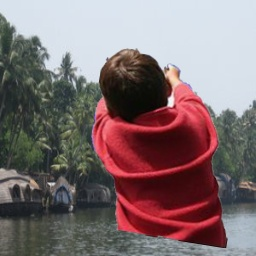
\includegraphics[width=0.1\textwidth]{syn1}};


%Lines
%% \draw[-strongT, line width=0.35mm] (input.east) -- (encoder.west);
\draw[->] (input.east) -- (encoder.west);
%% \draw (encoder.south) node[label=below:$b_1$,draw]{}
\draw[->] ($(encoder.east)+(0,0.3)$) |- ++(.5,0.0) -- ++(0, 1) |- (std.west);
\draw[->] ($(encoder.east)+(0,-0.3)$) |- ++(.5,-0.0) -- ++(0, -1) |- (mean.west);
\draw[->] (mean.east) |- ++(.5,-0.0) -- ++(0, 0.0) |- ($(latent.west)+(0, -0.3)$);
\draw[->] (std.east) |- ++(.5,-0.0) -- ++(0, -0.0) |- ($(latent.west)+(0, 0.3)$);
\draw[->] (latent.east) -- (decoder.west);
\draw[->] (decoder.east) -- (output.west);
%% \draw[->] (decoder.west) .. controls +(down:7mm) and +(right:7mm) .. (lowercircle.east);
%% \draw[->] (decoder.west) 

\end{tikzpicture}
%% \end{figure}

\end{document}
